\chapter{Results}
\label{ch:Results}
\thispagestyle{empty}

%%%%%%%%%%%%%%%%%%%%%%%%%%%%%%%%%%%%%%%%%%%%%%%%%%%%%%%%%%
%%%%%%%%%%%%%%%%%%%%%%%%%%%%%%%%%%%%%%%%%%%%%%%%%%%%%%%%%%
%%%%%%%%%%%%%%%%%%%%%%%%%%%%%%%%%%%%%%%%%%%%%%%%%%%%%%%%%%

As discussed, the goal of this study was to determine methods for atomic layer deposition of ferroelectric oxides. In the process of realizing this goal there were a number of different areas of study. The first is the analysis of thermal and chemical behavior of the various potential precursors, during which TGA and DSC were primarily used (see~\vref{sec:Methods-Thermal}). Secondly,  the analysis of the film growth behavior under various conditions, this was primarily measured and analyzed using the ellipsometric techniques discussed earlier (see~\vref{sec:Methods-Ellip}). Third, the film deposition needed to be tuned to produce films with a stoichiometric composition, as this was expected to produce films which would crystallize into the desired perovskite phase, see section~\vref{sec:Methods-Comp} for the methods used for this characterization. Fourth, the phase of the crystallized film was analyzed in detail to determine behavior of the films post-annealing. XRD was used extensively for this task (see~\vref{sec:Methods-XRD}).


%%%%%%%%%%%%%%%%%%%%%%%%%%%%%%%%%%%%%%%%%%%%%%%%%%%%%%%%%%
%%%%%%%%%%%%%%%%%%%%%%%%%%%%%%%%%%%%%%%%%%%%%%%%%%%%%%%%%%
%%%%%%%%%%%%%%%%%%%%%%%%%%%%%%%%%%%%%%%%%%%%%%%%%%%%%%%%%%

\section{Thermal Analysis}
\label{chap:Results-Thermal}

While a viable titanium precursor was well identified in literature as well as experimentally, as was the oxidizers that were used, there was no such universally accepted chemical used in ALD to provide a source of lead. The primary issue was either a lack of chemical stability or a undesirably low volatility in the compounds that currently were being used. TGA and DSC was performed on a number of potential candidates (see~\vref{sec:SampFab-Precursors} for more details) in order to gauge the performance of these materials. 

%%%%%%%%%%%%%%%%

\subsection{Thermogravimetric Analysis}

Thermogravimetric analysis allows for the estimation and comparison of volatility between multiple samples. It was used in this study primarily to compare properties of the two candidate precursors, \HFAc{} and \TMHD{}. Of primary consideration was the volatility of the compound --- evaluated qualitatively by analyzing the mass loss at various temperatures --- and whether or not there are indications of imperfect evaporation. The data collected for these materials can be found below. 

By analyzing the TGA curve for \HFAc{}, found in figure~\vref{fig:TGA-HFAc-Weight}, there are a number of features that are immediately noticeable. First of these is the presence of multiple stages of evaporation in the curve. These occur at approximately 170 and 190\degC{}. A TGA curve for a material that is purely evaporative, e.g. pure water, will have a smooth curve. Additional steps indicate that other processes are activating, and causing changes to the compound affecting the mass loss. 

More detail can be seen by performing a derivation on the TGA curve, giving the mass loss rate. This plot can be found in figure~\vref{fig:TGA-HFAc-DWeight}. This plot shows a shoulder on the primary evaporative peak, and then another peak starting at around 170\degC{} and peaking at 190\degC{}. The shoulder indicates that even during the evaporation of the bulk of the material, before residues and other imperfections cause rate changes, a secondary mechanism is activating and impacting the mass loss rate. 

\begin{figure}[tbp]
   \centering
   \subfloat[Mass vs. Temperature][Mass vs. Temperature]{%
   	\label{fig:TGA-HFAc-Weight}%
	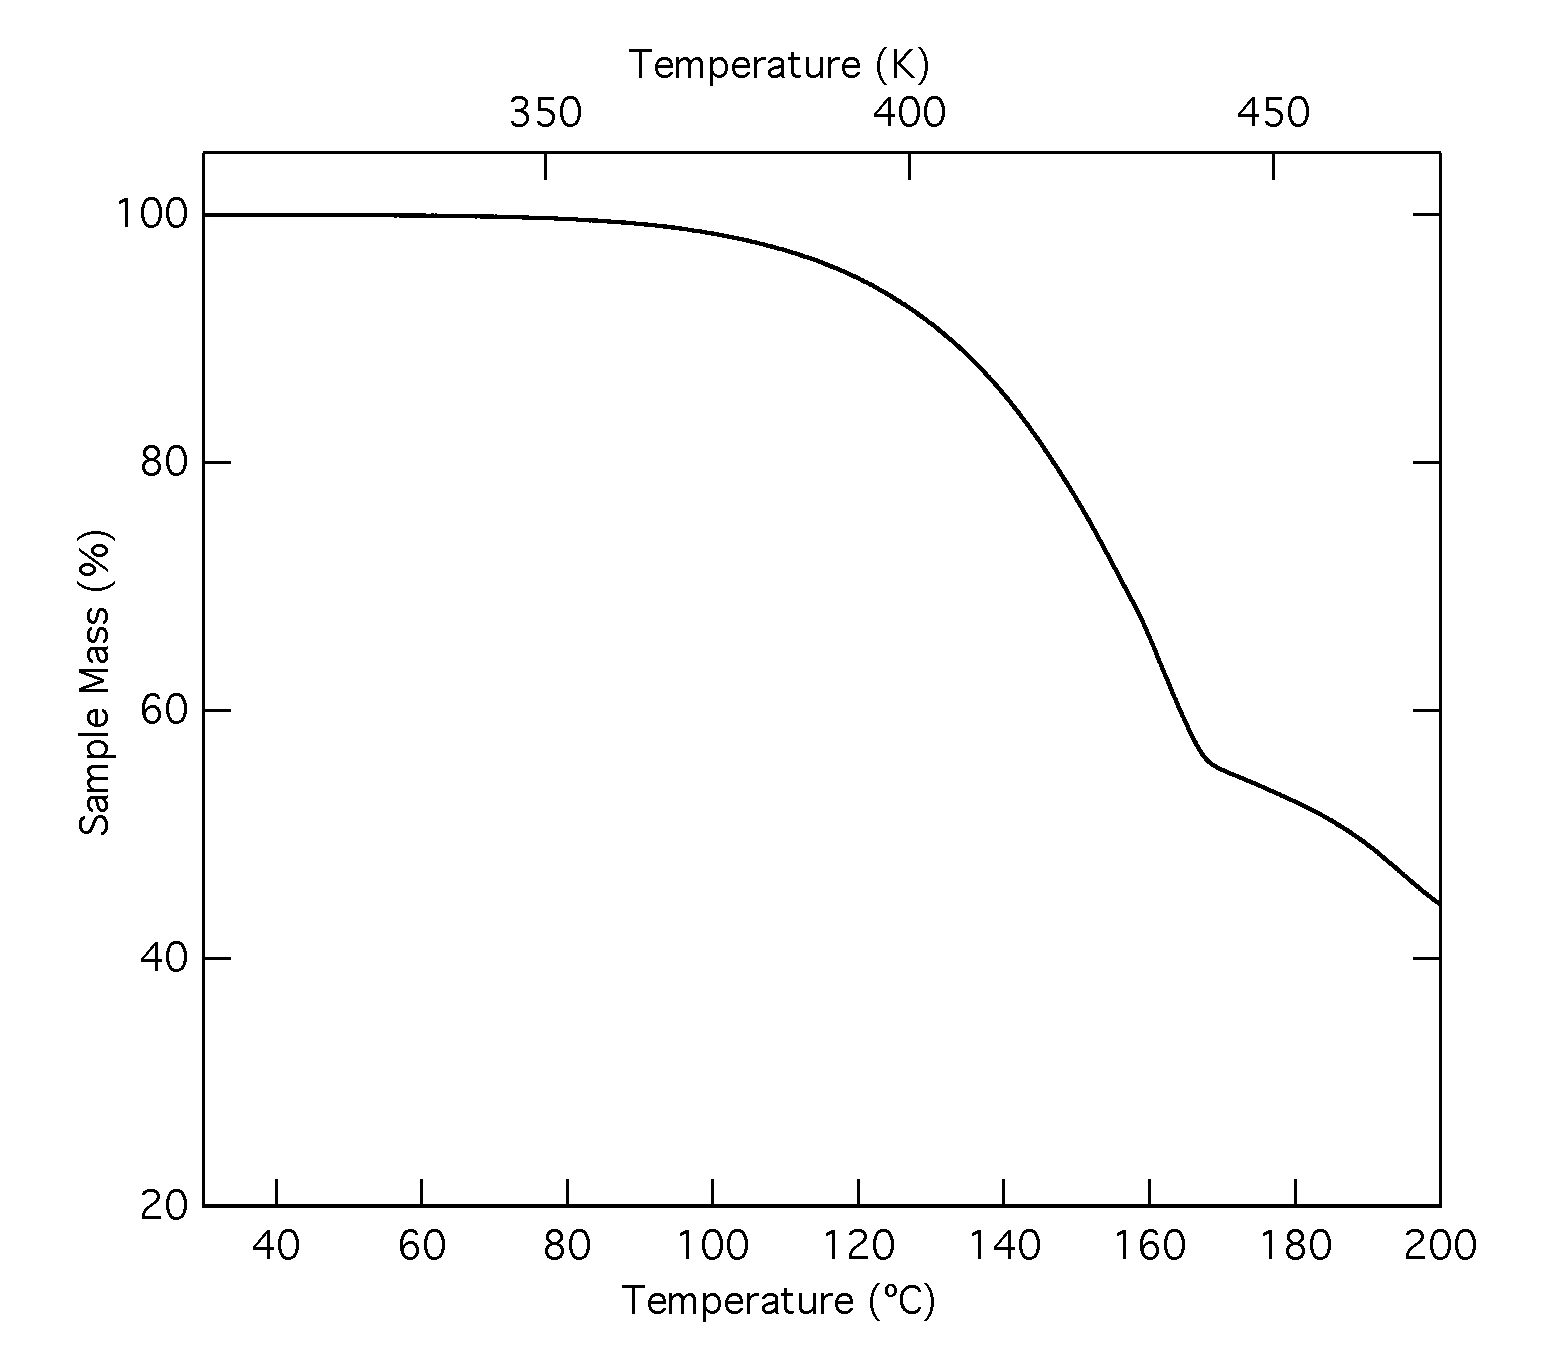
\includegraphics[width=0.45\textwidth]{./Figures/Data/Thermal-Analysis/TGA/HFAc-Weight}%
	}
	\hspace{1cm}
  \subfloat[Derivative of Mass vs. Temperature][Derivative of Mass vs. Temperature]{%
   	\label{fig:TGA-HFAc-DWeight}%
	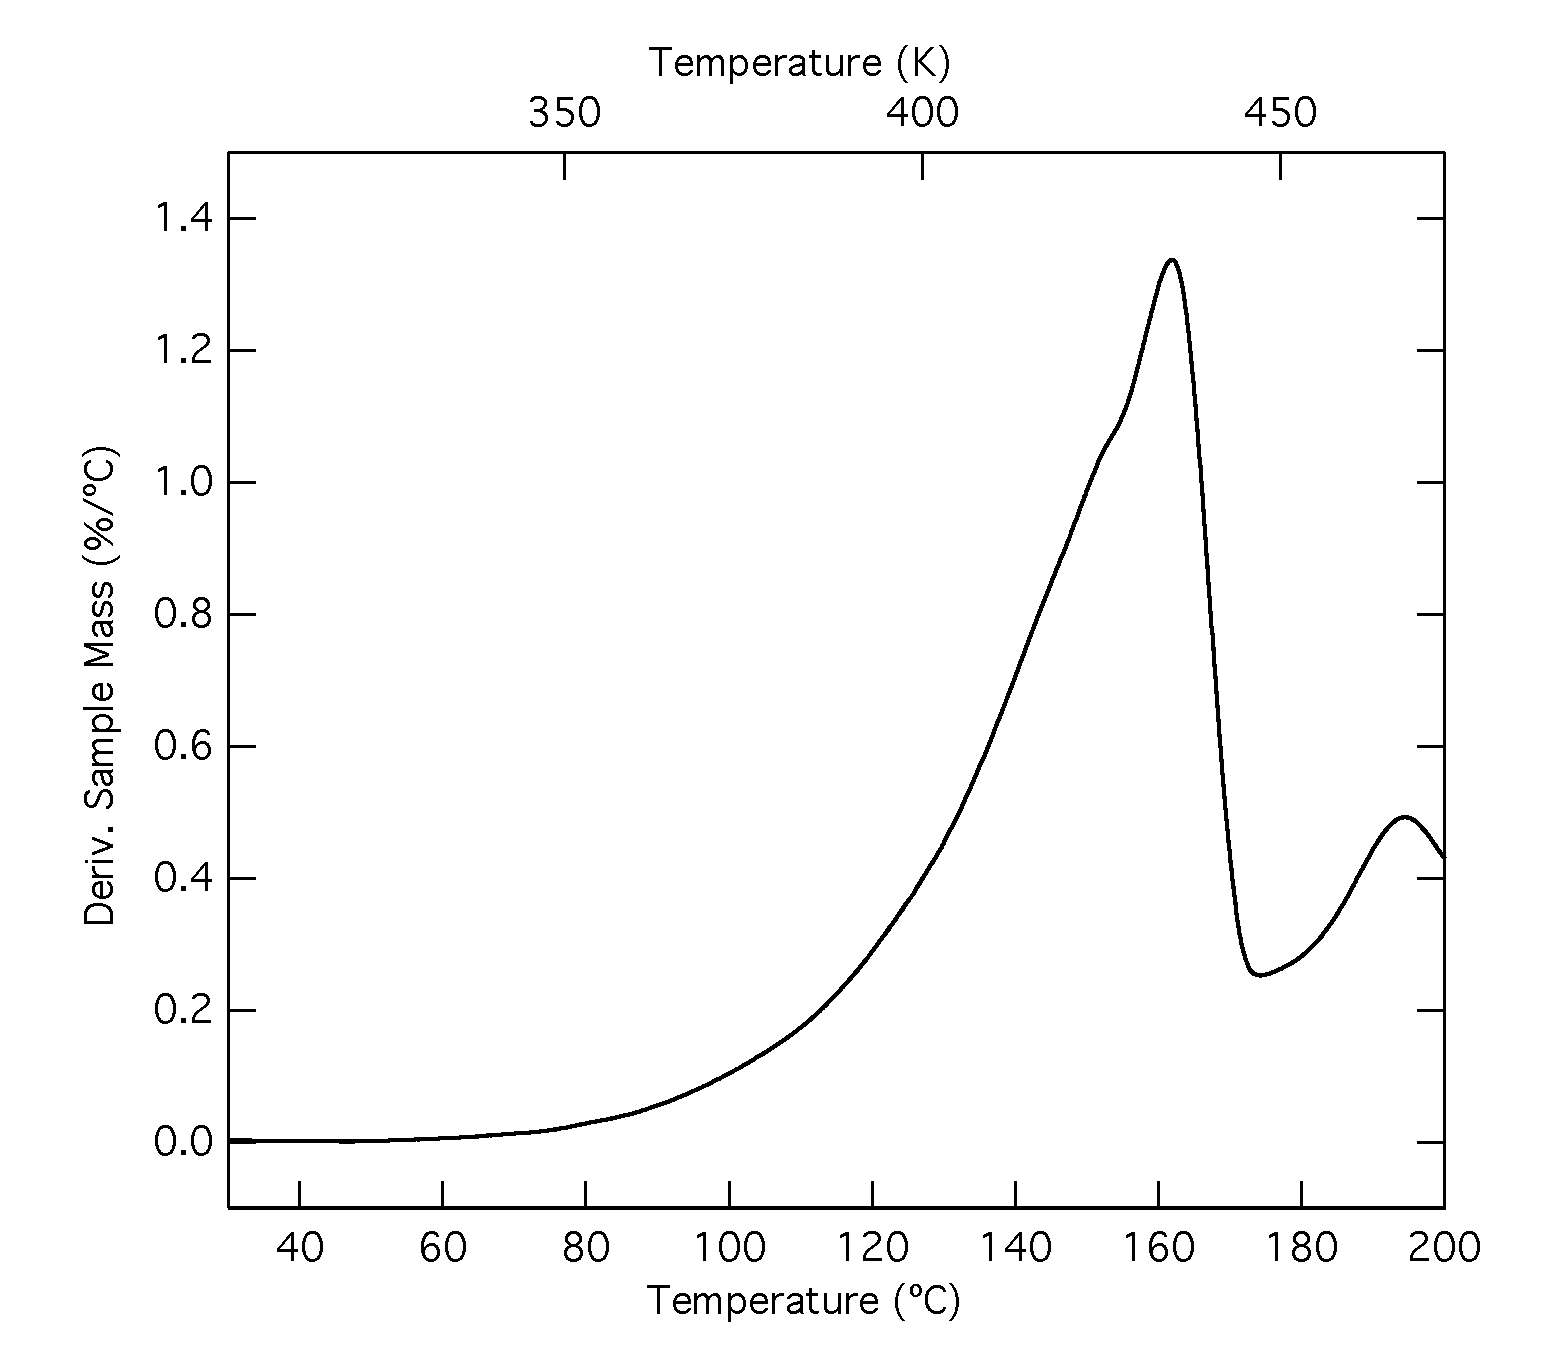
\includegraphics[width=0.45\textwidth]{./Figures/Data/Thermal-Analysis/TGA/HFAc-DWeight}%
	} 	
   \caption[TGA Results for Pb(HFAc)$_{2}$ Precursor]%
   		{Plots of the results from TGA experiments on Pb(HFAc)$_{2}$. The plot shown in (a) gives the raw %
		data showing the current mass as a function of temperature. (b) gives the same data, transformed %
		to show the derivative of mass. Thus (b) shows the rate of mass loss at a given temperature. Initial %
		sample mass: 6.092 mg}
   \label{fig:TGA-HFAc}
\end{figure}

Comparing this data with that of \TMHD{}, it is immediately obvious that the evaporation mechanism for the latter is much smoother. There is no major visible step, apart from some slight changes nearing the upper end of the testing temperature range (185--200\degC{}). With a closer look at figure~\vref{fig:TGA-TMHD-DWeight}, it is easier to see that there is basically smooth vaporization up to approximately 180\degC{}, at which point the evaporation is slowed dramatically due to residue buildup. 

\begin{figure}[tbp]
   \centering
   \subfloat[Mass vs. Temperature][Mass vs. Temperature]{%
   	\label{fig:TGA-TMHD-Weight}%
	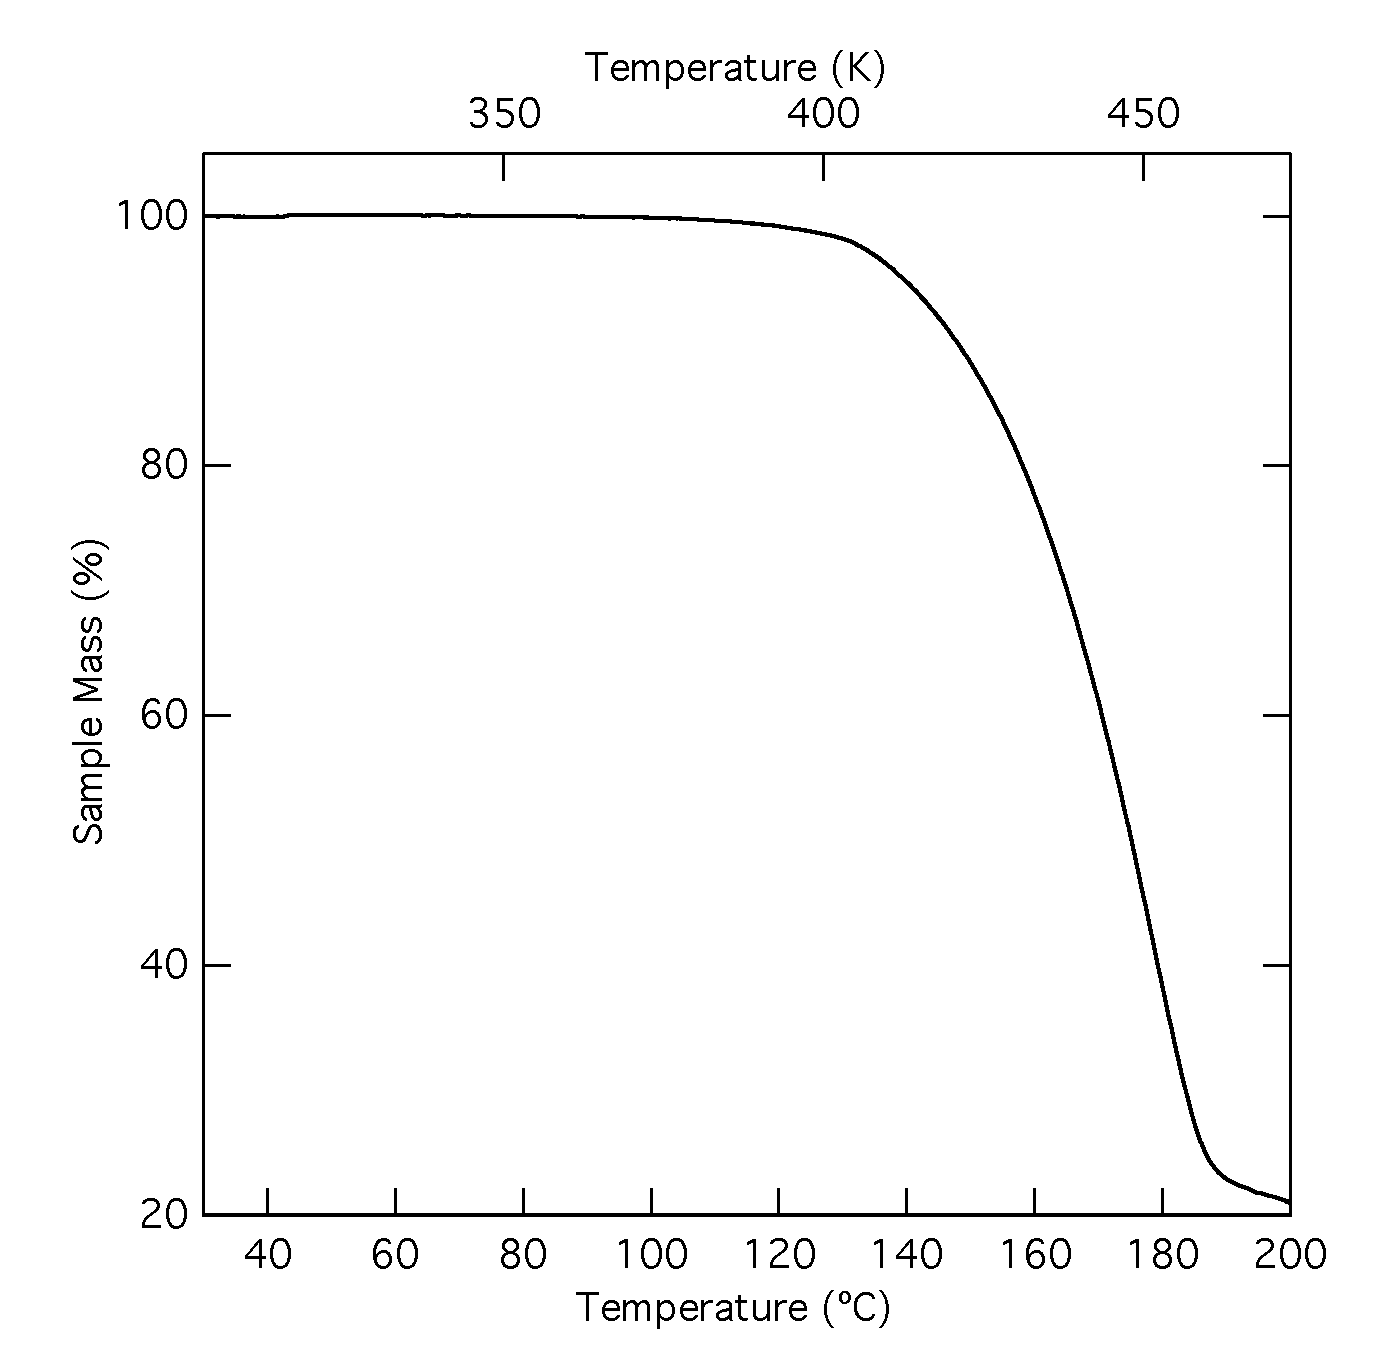
\includegraphics[width=0.45\textwidth]{./Figures/Data/Thermal-Analysis/TGA/TMHD-Weight}%
	}
	\hspace{1cm}
  \subfloat[Derivative of Mass vs. Temperature][Derivative of Mass vs. Temperature]{%
   	\label{fig:TGA-TMHD-DWeight}%
	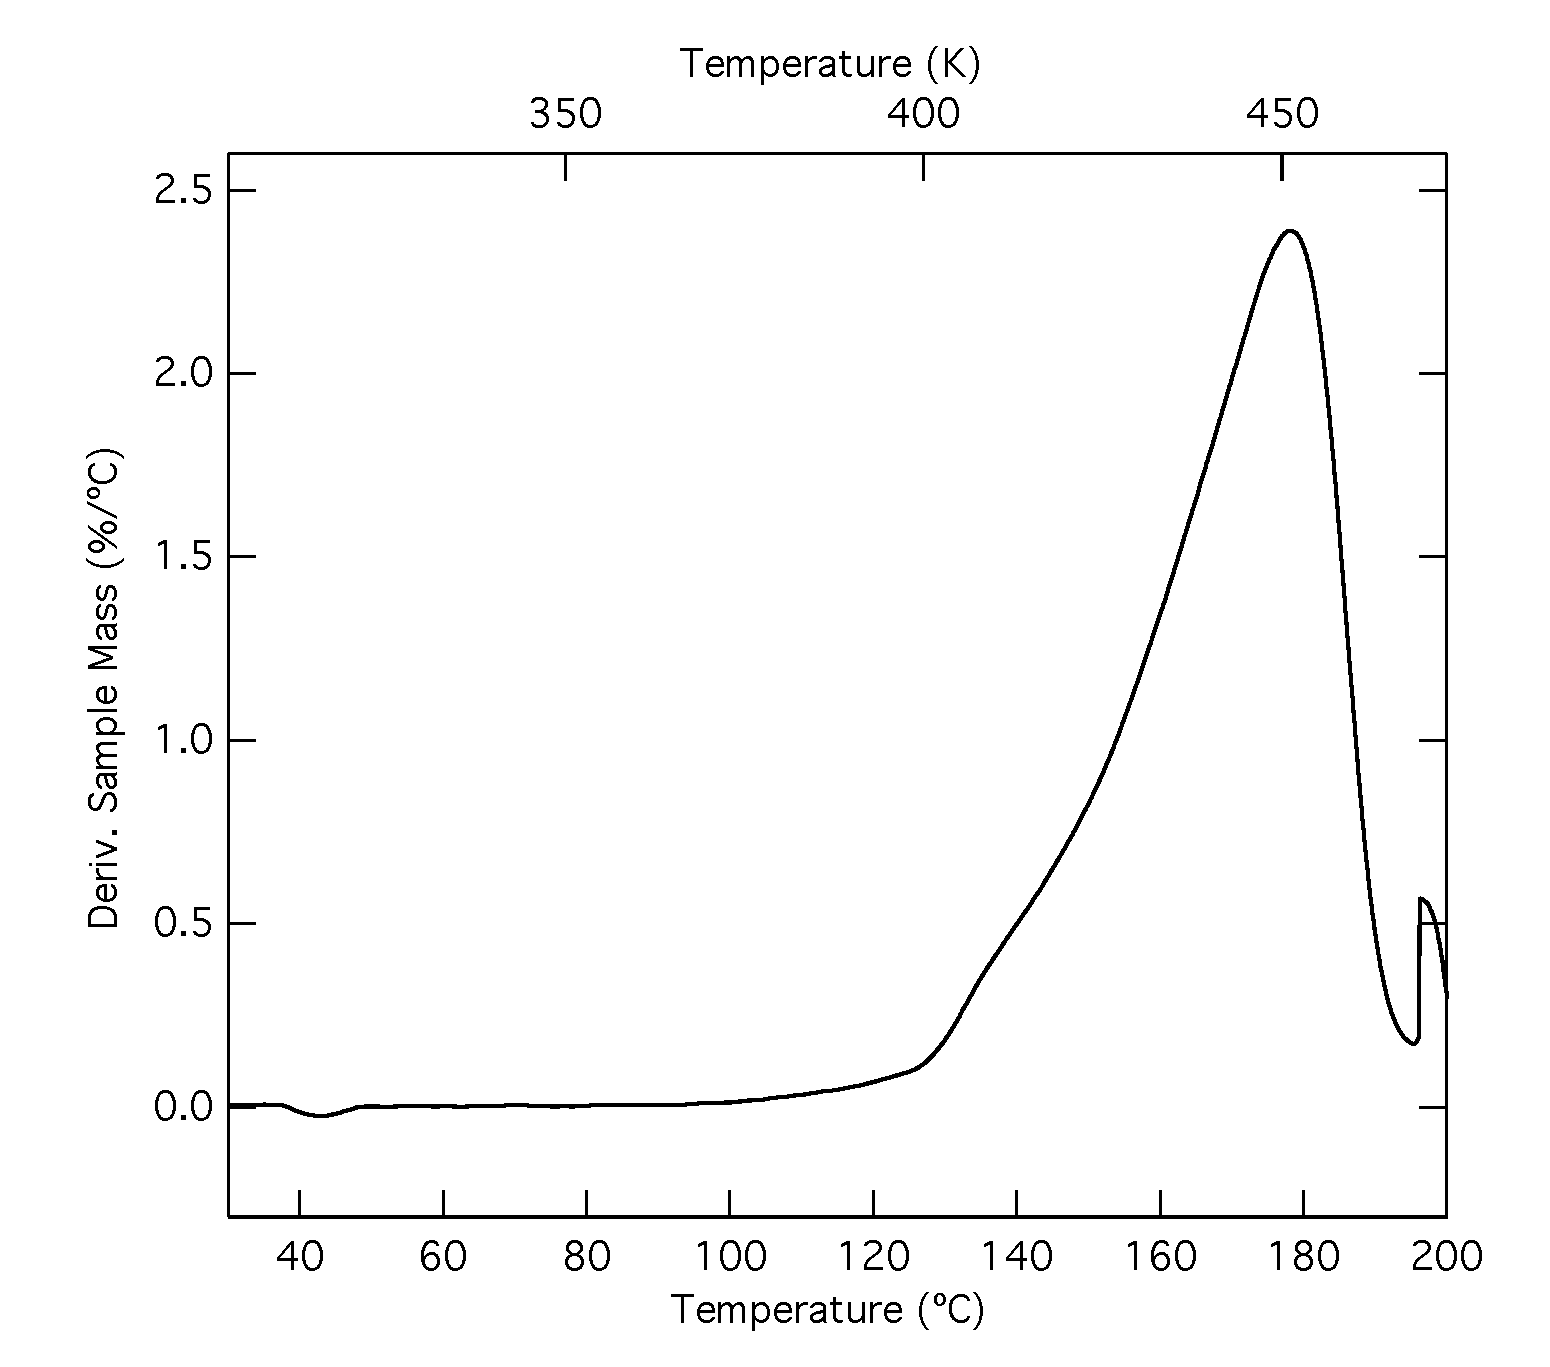
\includegraphics[width=0.45\textwidth]{./Figures/Data/Thermal-Analysis/TGA/TMHD-DWeight}%
	} 	
   \caption[TGA Results for Pb(HFAc)$_{2}$ Precursor]%
   		{Plots of the results from TGA experiments on Pb(TMHD)$_{2}$. As in figure~\vref{fig:TGA-HFAc}, (a) %
		presents the actual mass as a function of temperature, while (b) gives the derivative of that function. %
		Initial sample mass: 3.719 mg}
   \label{fig:TGA-TMHD}
\end{figure}

Neither of these precursors evaporated cleanly, leaving residues of more than 20\% of their initial sample mass during the temperature scanning tests discussed above. When these were tested at moderate temperatures, such as those to be used for evaporation in the ALD system, both left even larger fractions of their initial masses behind. Testing at a constant temperature (160\degC{}) over a longer period of time gives the plots shown in figure~\vref{fig:TGA-Hold}. From this test, it was found that \HFAc{} left a much larger residue than \TMHD{}, 63\% and 34\% respectively. 

\begin{figure}[htbp]
   \centering
   \subfloat[\HFAc][\HFAc]{%
   	\label{fig:TGA-HFAc-Hold}%
	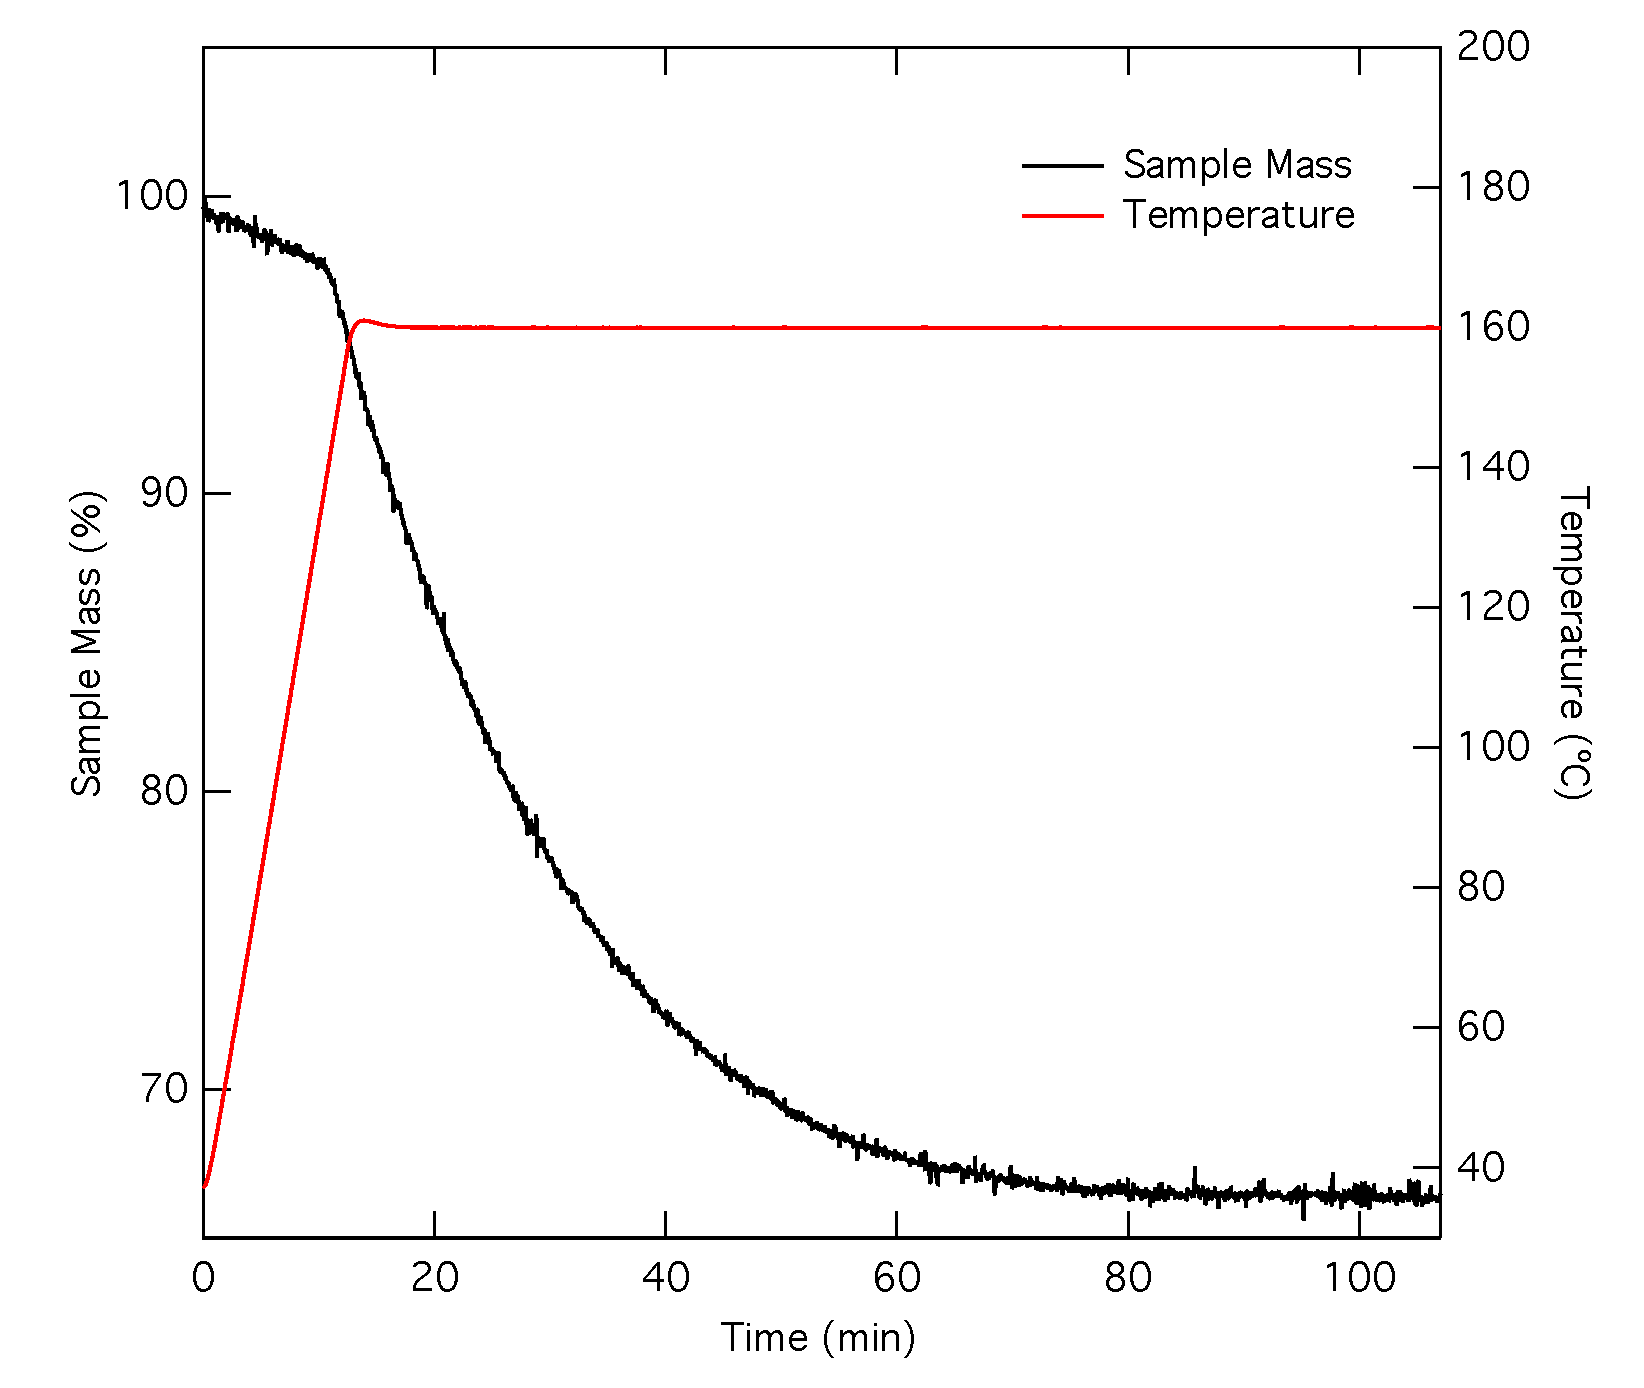
\includegraphics[width=0.45\textwidth]{./Figures/Data/Thermal-Analysis/TGA/HFAc-Hold}%
	}
	\hspace{1cm}
  \subfloat[\TMHD][\TMHD]{%
   	\label{fig:TGA-TMHD-Hold}%
	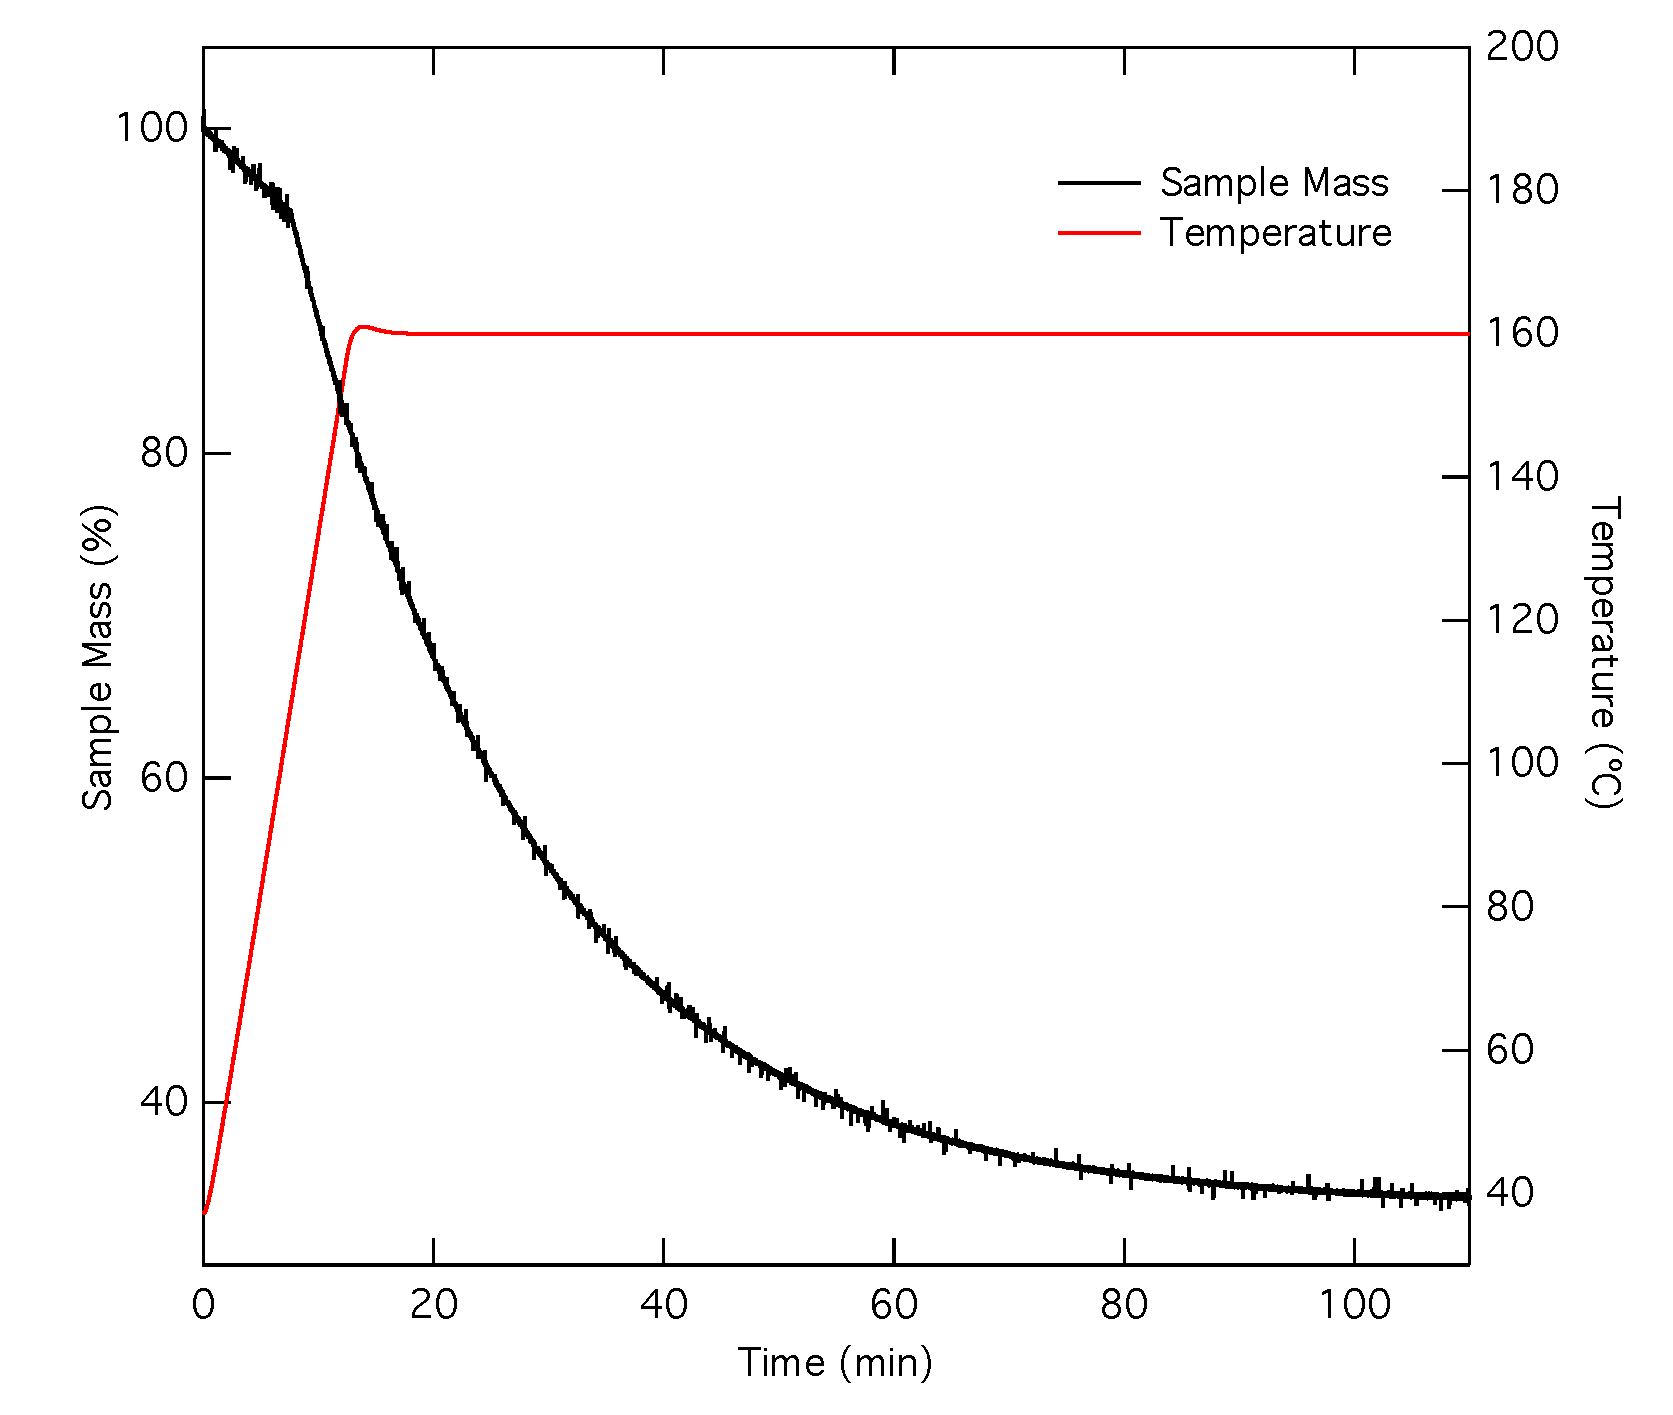
\includegraphics[width=0.45\textwidth]{./Figures/Data/Thermal-Analysis/TGA/TMHD-Hold}%
	} 	
   \caption[Constant Temperature TGA Experiments]%
   		{Plots of the results from ramp-and-hold TGA experiments designed to investigate residual material %
		after complete evaporation at a given temperature. From the TGA experiments seen above (figs.~%
		\vref{fig:TGA-HFAc} and \vref{fig:TGA-TMHD}), a common temperature of 160\degC{} was chosen %
		for this experiment. Sample masses were 3.921 mg and 4.381 mg for \HFAc{} and \TMHD{} respectively.}
   \label{fig:TGA-Hold}
\end{figure}

Based on the results of these tests, the lower residual mass and the cleaner evaporative process, \TMHD{} was predicted to have better performance as an ALD precursor. 

%%%%%%%%%%%%%%%%

\subsection{Differential Scanning Calorimetry}

As discussed in previous chapters, DSC is a powerful tool for analyzing the behavior of precursors. The data collected allows for the understanding of various energies in the material. 

When considering the energetic behavior of \HFAc{} (see fig.~\vref{fig:DSC-HFAc}), there are a few minor features that can be noticed. Primarily at 25 and 150\degC{} small peaks are visible that indicate changes in the material other than the solid to liquid phase change, which is the much larger peak seen around 155-160\degC{}. However, these peaks appear to be negligible, as the total energy release by the sample is a mere 5.32 mJ (1.13 J/g), which is too low for any major chemical changes to be occurring. 

\begin{figure}[htb]
	\centering
	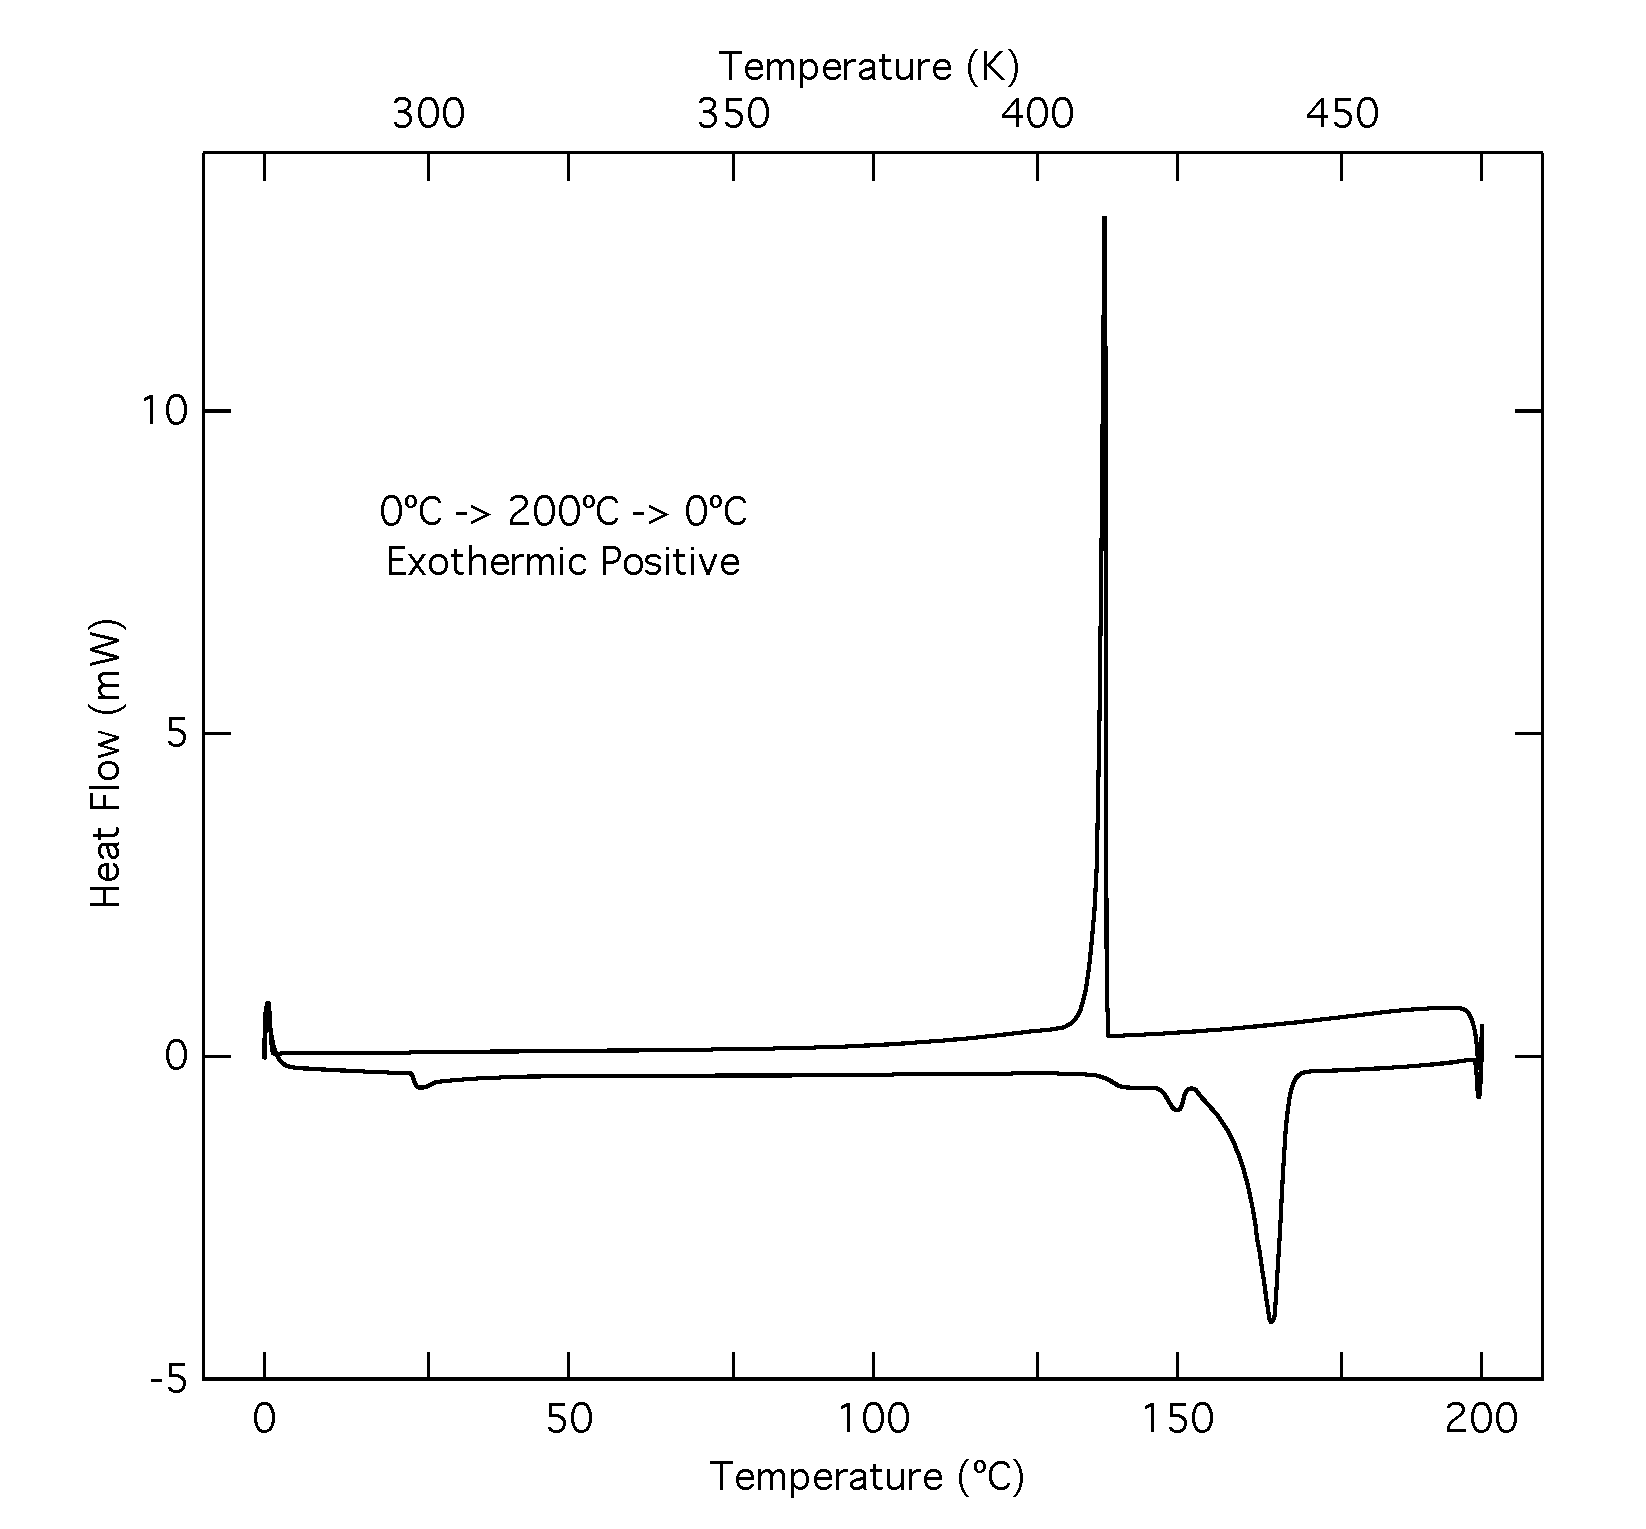
\includegraphics[width=0.66\textwidth]{./Figures/Data/Thermal-Analysis/DSC/HFAc}
	\caption[DSC Results of \HFAc{}]%
		{Plot of the DSC scan of \HFAc{}. In this plot exothermic behavior, where the sample releases heat, is %
		considered positive. Thus, the first sweep of the scan (from 0\degC{} to 200\degC{}) is negative. %
		Sample mass: 4.7 mg.}
	\label{fig:DSC-HFAc}
\end{figure}

Similarly, when \TMHD{} is heated to moderate temperatures (up to 200\degC{}, see fig~\vref{fig:DSC-TMHD-200}), such as those used in the evaporation and transport stages of the ALD system, there are no irregularities in the data. There is also no net energy gain or loss during the test indicating that heating up to 200\degC{}, along with the associated melting and freezing of the compound, is not detrimental to its structure. 

If the test is again performed, but with a higher upper temperature bound, the data is drastically different (see fig.~\vref{fig:DSC-TMHD-300}). As the sample is heated up to 300\degC{}, there are a number of significant energy releases that occur. These processes initiate at 234\degC{}, and are due to the precursor undergoing pyrolysis reactions. As such, this sets the safe upper temperature range for the ``ALD window'' of \TMHD{} at 230\degC{}. ALD reactions require that the precursor arrive to the surface intact and only react with surface species present. 

\begin{figure}[tbp]
	\centering
	\subfloat[][Low Temperature Test (30--200--30\degC{})]{\label{fig:DSC-TMHD-200}%
		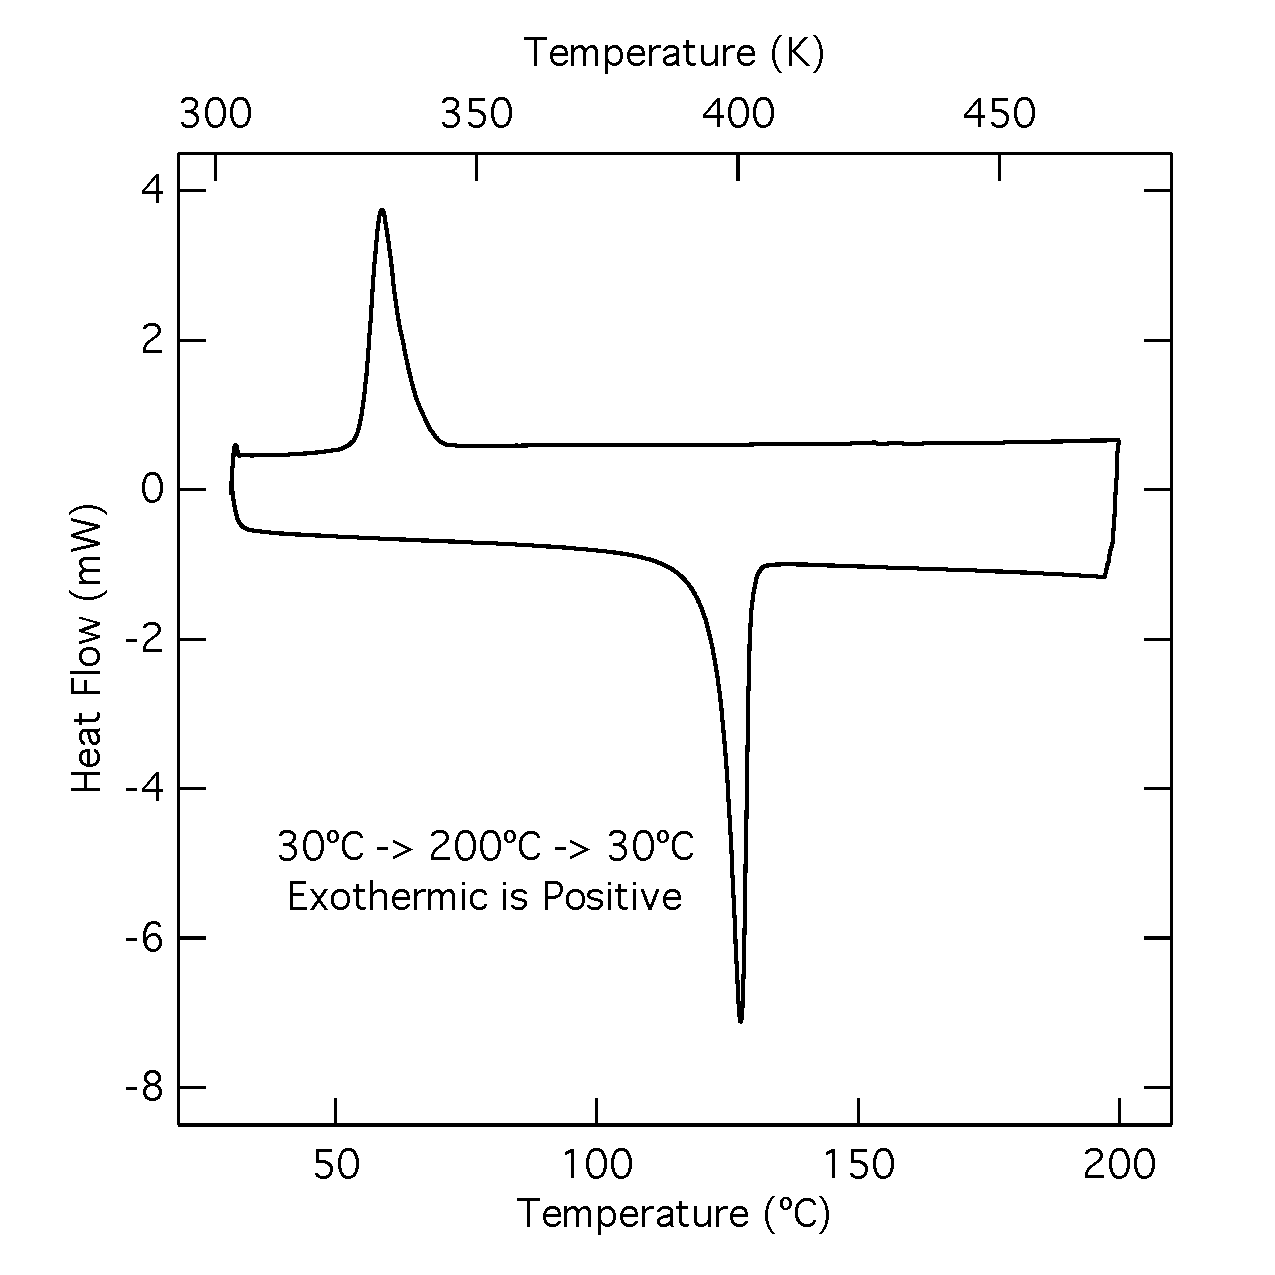
\includegraphics[width=0.66\textwidth]{./Figures/Data/Thermal-Analysis/DSC/TMHD-200}%
		}\\
	%\hspace{0.5cm}
	\subfloat[][High Temperature Test (30--300-30\degC{})]{\label{fig:DSC-TMHD-300}%
		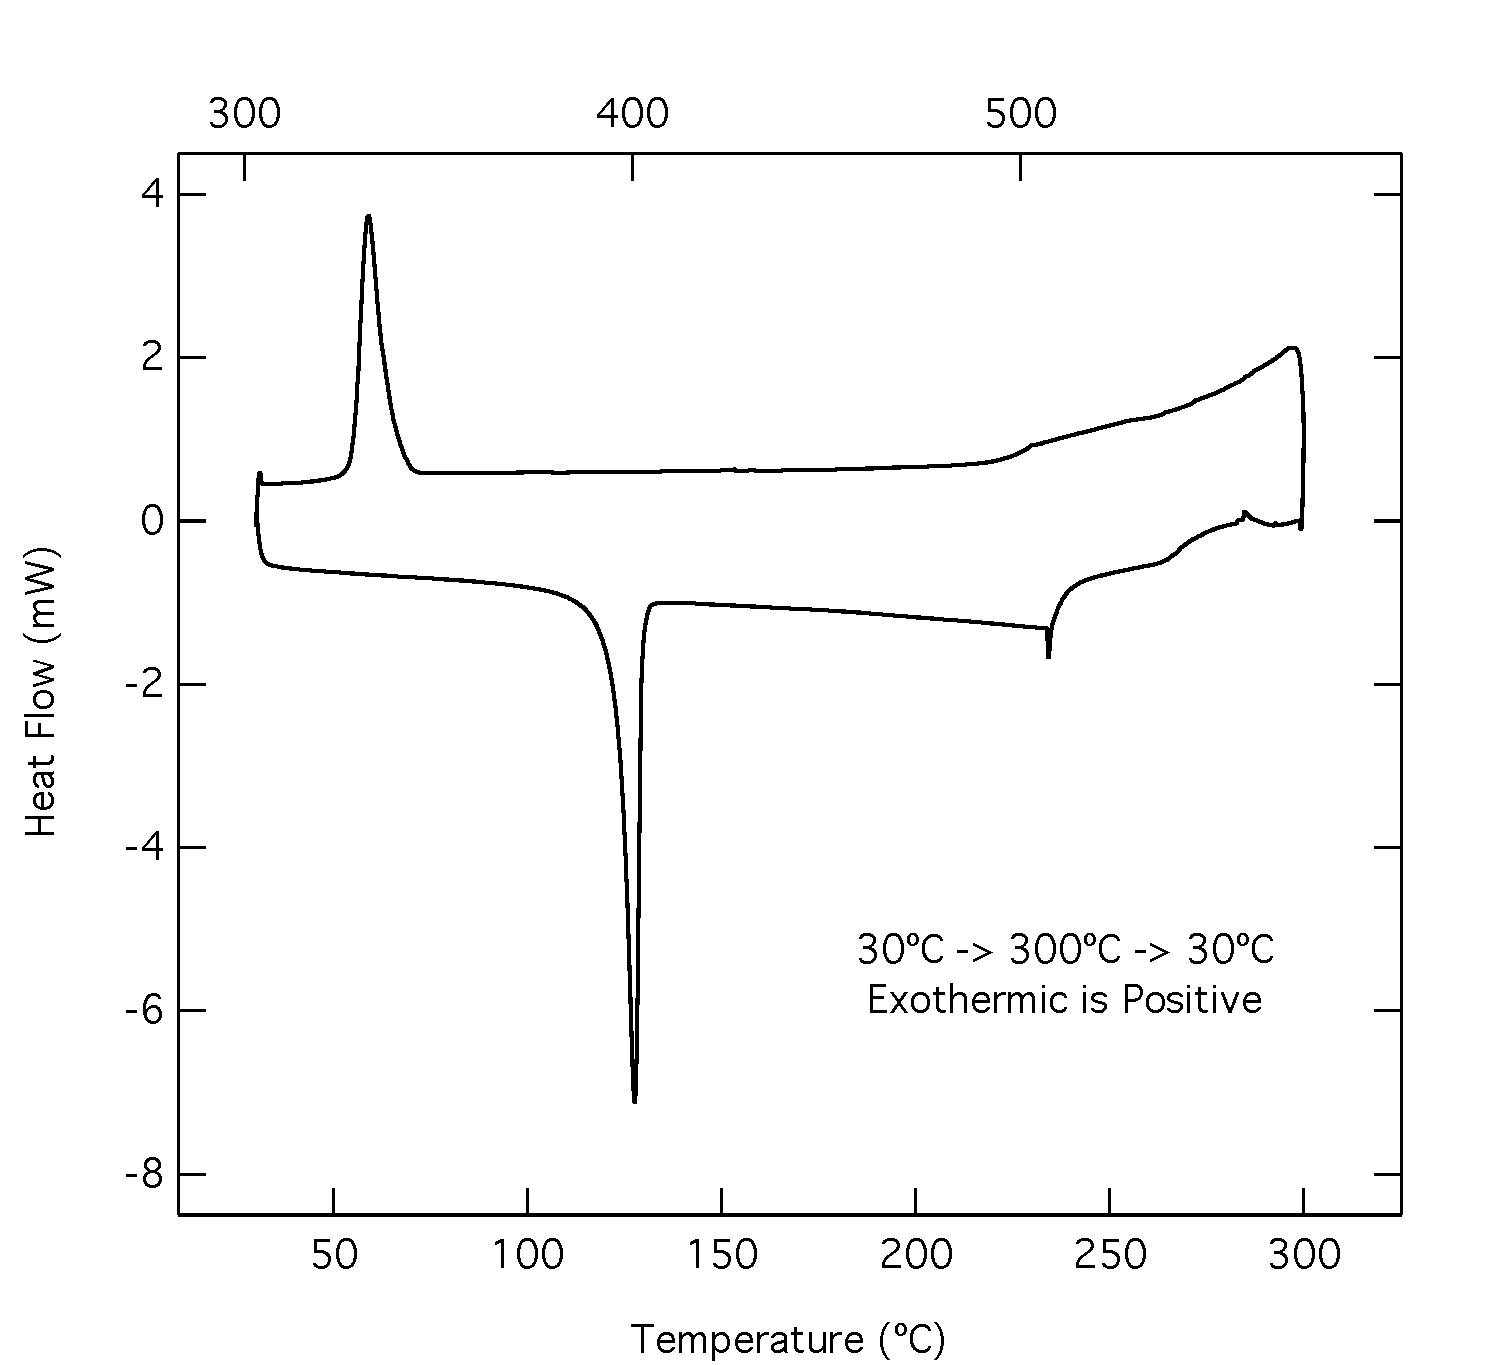
\includegraphics[width=0.66\textwidth]{./Figures/Data/Thermal-Analysis/DSC/TMHD}%
		}
	\caption[DSC Results of \TMHD{}]%
		{Results from the DSC scans of \TMHD{}. (a) Temperatures up to 200\degC{} show no change in the %
		material other than that of melting and freezing. (b) As temperatures increase, features start to appear %
		indicating chemical reconfiguration of the molecule.}
	\label{fig:DSC-TMHD}
\end{figure}
\clearpage
%%%%%%%%%%%%%%%%%%%%%%%%%%%%%%%%%%%%%%%%%%%%%%%%%%%%%%%%%%
%%%%%%%%%%%%%%%%%%%%%%%%%%%%%%%%%%%%%%%%%%%%%%%%%%%%%%%%%%
%%%%%%%%%%%%%%%%%%%%%%%%%%%%%%%%%%%%%%%%%%%%%%%%%%%%%%%%%%

\section{List of Samples}
\label{chap:Results-Samples}

Based on the results from the thermal analysis, a number of samples were deposited with various deposition parameters. Information on the deposition parameters for each of the samples used in this study can be found in the following table~\vref{tbl:LoSamples}. A small number of samples were attempted at 200\degC{}, but it was quickly determined that 225\degC{} provided better growth behavior without risking thermal cracking of the compound. 

{\small
\begin{longtable}{ccccccccc}
	\caption[List of Samples]{A list of samples produced during the course of this project.%
	\label{tbl:LoSamples}}\\
	\toprule
	&&&&&\multicolumn{3}{c}{Annealing}&\\ \cmidrule{6-8}
	Temp.		&Run \#	&Pb:Ti	 	&Cycles 	&Subs. 	&Type	&Temp. 		&Time &XRD\\ 
	(\degC{})		&		&Ratio		&		&Type	&		&(\degC{})	&(min) &\\ \midrule%
	\endfirsthead
	\caption[]{A list of samples used during the course of this project.}\\
	\toprule
	&&&&&\multicolumn{3}{c}{Annealing}&\\ \cmidrule{6-8}
	Temp.		&Run \#	&Pb:Ti	 	&Cycles 	&Subs. 	&Type	&Temp. 		&Time &XRD\\ 
	(\degC{})		&		&Ratio		&		&Type	&		&(\degC{})	&(min) &\\ \midrule%
	\endhead
	200	&3		&1:1		&250	&Si		&None	&N/A		&N/A		&No\\
		&2		&1:2		&250	&Si		&None	&N/A		&N/A		&No\\
		&30		&3:1		&160	&Si		&None	&N/A		&N/A		&No\\
		&		&		&		&Pt-Si	&None	&N/A		&N/A		&No\\ \midrule
	225	&0		&1:1		&625	&Si		&Oven	&650	&120	&Yes\\
		&		&		&		&		&Oven	&900	&120	&Yes\\
		&		&		&		&		&RTA	&900	&10		&No\\
		&1		&1:1		&475	&Si		&None	&N/A		&N/A		&No\\
		&6		&1:2		&250	&Si		&None 	&N/A		&N/A		&No\\
		&13		&3:1		&250	&Si		&None 	&N/A		&N/A		&No\\
		&16		&3:1		&150	&Si		&RTA	&650	&1		&No\\
		&19		&3:1		&100	&Si		&None 	&N/A		&N/A		&No\\
		&		&		&		&Pt-Si	&None 	&N/A		&N/A		&No\\
		&20		&3:1		&200	&Si		&None 	&N/A		&N/A		&No\\
		&		&		&		&Pt-Si	&Oven	&650	&90		&Yes\\
		&		&		&		&STO	&Oven	&650	&90		&No\\
		&21		&3:1		&150	&Si		&None 	&N/A		&N/A		&No\\
		&		&		&		&Pt-Si	&Oven	&650	&90		&No\\
		&		&		&		&STO	&Oven	&650	&90		&No\\
		&22		&3:1		&150	&Si		&None 	&N/A		&N/A		&No\\
		&		&		&		&Pt-Si	&Oven	&650	&90		&Yes\\
		&23		&3:1		&200	&Si		&None 	&N/A		&N/A		&No\\
		&		&		&		&Pt-Si	&Oven	&650	&90		&Yes\\
		&28		&3:1		&120	&STO	&Oven	&650	&90		&Yes\\
	\bottomrule
\end{longtable}}

%%%%%%%%%%%%%%%%%%%%%%%%%%%%%%%%%%%%%%%%%%%%%%%%%%%%%%%%%%
%%%%%%%%%%%%%%%%%%%%%%%%%%%%%%%%%%%%%%%%%%%%%%%%%%%%%%%%%%
%%%%%%%%%%%%%%%%%%%%%%%%%%%%%%%%%%%%%%%%%%%%%%%%%%%%%%%%%%

\section{Ellipsometry}
\label{chap:Results-Ellipsometry}

Ellipsometry was a valuable tool during the course of this study. As discussed previously, it is capable of quickly, accurately, and non-destructively determine various properties of thin film layer stacks. Of primary importance is the ability of the tool to provide a rapid method of determining the thickness of a deposited layer. In ALD the growth rate is one of the primary markers of a well-tuned deposition process. An uncontrollably high growth rate is nearly as detrimental as having minimal growth. Varying deposition parameters and noting their effects on the growth rate of the process provided valuable insight into how best to tune the process. 

Given in table~\ref{tbl:LoThicknesses} is information on various samples and their as-deposited layer thicknesses, along with some relevant deposition parameters. One can also see from the plot of the sample thicknesses with respect to the number of deposition cycles (fig.~\vref{fig:Ellip-rates}) the consistency of a growth rate given a certain set of parameters. There is a small number of initial cycles required to initiate growth, referred to as ``incubation'' cycles, and then the film thickness follows a close linear dependence to the number of deposition cycles. This is indicative of a deposition that is operating within the ALD window and behaving well. From figure~\ref{fig:Ellip-rates} it was found that films deposited on silicon required approximately 10 cycles to initiate layer growth and subsequently grew at a rate of 3.78 \AA/cycle. For platinum coated silicon the incubation time was longer, an average of 36 cycles, but the films grew at a faster rate of 4.12 \AA/cycle. On STO crystals a 21 cycle incubation period was followed by a growth phase with a rate of 4.08 \AA/cycle. This varies greatly from values reported in table~\ref{tbl:LoThicknesses} as the growth rates reported here do not take into account the incubation time. The relatively constant number of initiation cycles has a seemingly greater effect on samples with low cycle counts; the incubation cycles take up a greater percentage of the total run and lower the growth rate accordingly. 

\begin{table}[tbp]
	\centering
	\small
	\caption[Sample Thicknesses and Growth Rates]%
		{Table of the film thicknesses and associated growth rates as measured by ellipsometry. Growth rates do %
		not take into account any incubation times for the films.}
	\label{tbl:LoThicknesses}
	\begin{tabular}{llllrr}
		\toprule
		Pb:Ti		&Sample	&Cycles		&Substrate	&Thickness	&Growth Rate	\\
		Ratio	&\#		&			&Type		&(nm)		&(\AA/cycle)	\\ \midrule
		1:1		&0		&625		&Si			&85.9		&1.37		\\
				&1		&475		&Si			&63.4		&1.33		\\
		3:1		&13		&250		&Si			&*32.9		&*1.31		\\
				&16		&150		&Si			&51.2		&3.41		\\
				&19		&100		&Si			&34.3		&3.43		\\
				&		&			&Pt-Si		&27.5		&2.75		\\
				&20		&200		&Si			&71.8		&3.59		\\
				&		&			&Pt-Si		&64.4		&3.22		\\
				&		&			&STO		&73.6		&3.68		\\
				&21		&150		&Si			&53.2		&3.54		\\
				&		&			&Pt-Si		&45.8		&3.05		\\
				&		&			&STO		&52.9		&3.53		\\
				&22		&150		&Si			&53.3		&3.55		\\
				&		&			&Pt-Si		&46.5		&3.10		\\
				&23		&200		&Si			&72.0		&3.60		\\
				&		&			&Pt-Si		&64.6		&3.23		\\
				&28		&120		&STO		&41.0		&3.42		\\	
		\bottomrule
	\end{tabular}
\end{table}

\begin{figure}[htbp]
	\centering
	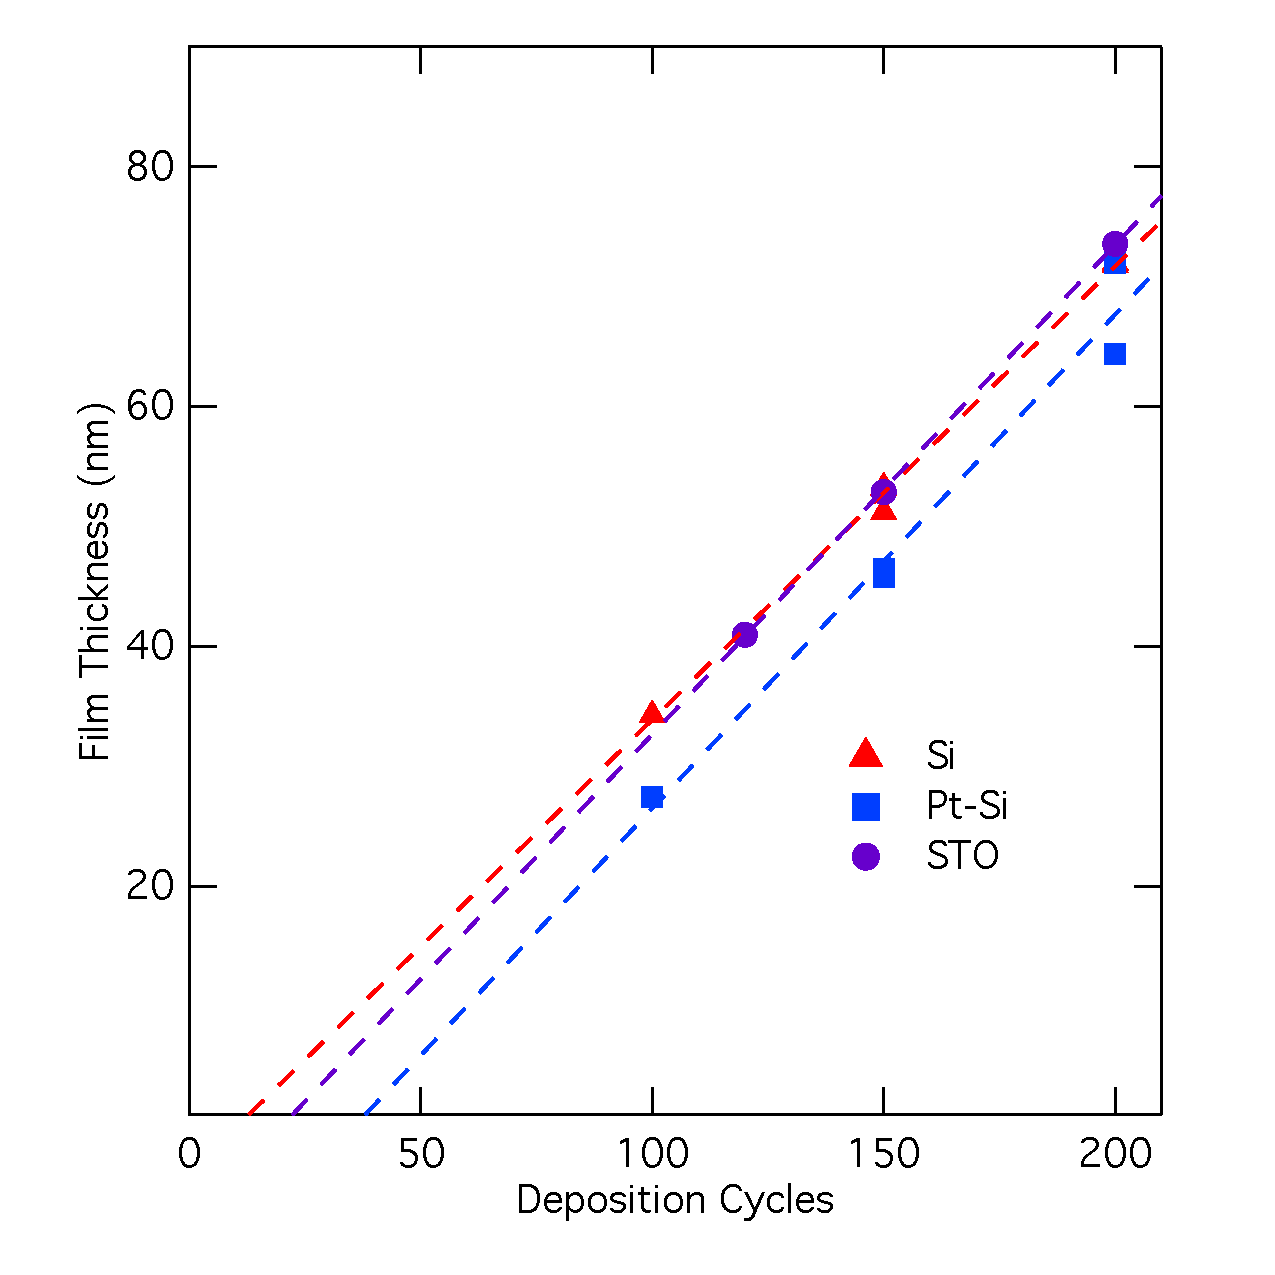
\includegraphics[width=0.6\textwidth]{./Figures/Data/Ellipsometry/Ellip-Rates}
	\caption[Film Thicknesses vs. Deposition Cycles]%
		{A plot of film thicknesses determined by ellipsometry. Growth rates and average incubation times are %
		extrapolated from this data. All films were deposited with a 3:1 Pb:Ti ratio and at 225\degC{}}
	\label{fig:Ellip-rates}
\end{figure}
	
An additional piece of information that can be extracted from ellipsometric analysis is an estimation of the band gap energy of the deposited layer. Because the final model used in the analysis method (see section~\vref{chap:Methods-Ellip-Analysis}) is physically descriptive of the optical properties of the material, it is possible to extract such information from the model. By transforming the plot of the extinction coefficient, $k$, into that of the absorption coefficient, $\alpha$, it becomes possible to use the method developed by Tauc, \emph{et.al.} \reword{[citation needed]} to determine the band gap energy of the material. However, such analysis does not take into account presence of multiple phases in the layer and takes a weighted average of the bandgaps. It also requires that the sample be properly crystallized, and thus must have undergone an annealing treatment before the analysis method becomes valid. However, since the samples produced here had low phase purity, which will be discussed in subsequent sections, this analysis was of little use as a film benchmark. 

%%%%%%%%%%%%%%%%%%%%%%%%%%%%%%%%%%%%%%%%%%%%%%%%%%%%%%%%%%
%%%%%%%%%%%%%%%%%%%%%%%%%%%%%%%%%%%%%%%%%%%%%%%%%%%%%%%%%%
%%%%%%%%%%%%%%%%%%%%%%%%%%%%%%%%%%%%%%%%%%%%%%%%%%%%%%%%%%

\section{Composition}
\label{chap:Results-Composition}

Controlling the composition of the film was another primary task during the course of this project. Controlling the stoichiometry of the deposited films was of critical importance in obtaining films that presented the perovskite phase. If the balance of the two cations (\PbIon{} and \TiIon{}) was allowed to stray away from unity, other phases would be preferred or a mixture of phases would precipitate during a crystallizing heat treatment.  

As discussed previously, X-ray fluorescence was the method used for performing the composition analysis of the film structures. Through testing it was found that a deposition ratio of 3:1 in favor of the lead half-reaction provided the best film composition; there were a pair of samples deposited at an even 1:1 ratio that also provided near unity compositions (sample \#0 and \#1). Table~\ref{tbl:XRF-compositions} provides a list of samples and their compositions measured via XRF. 

As mentioned in section~\ref{sec:Methods-XRF}, samples deposited on STO were unable to have their compositions accurately measured using this technique. This was due to the confounding influence of the titanium content in the STO substrate, and there were no surface sensitive characterization methods available. 


\begin{table}[htbp]
	\centering
	\caption[XRF Calculated Compositions]{Calculated compositions of selected samples, determined via XRF. \\Composition percentages are all $\pm$1\%.}\label{tbl:XRF-compositions}
	\begin{tabular}{l l r r r}
	\toprule
	&&\multicolumn{3}{c}{Composition (\%)}\\
	\cmidrule{3-5}
	Run \#&Substrate&Lead&Titanium&Ti:Pb Ratio\\
	\midrule
% 	Run	Sub-Type		Pb%		Ti%		Ti:Pb ratio
	0	&\ce{SiO2}	&56.0	&44.0	&0.786\\
	1	&\ce{SiO2}	&55.0	&45.0	&0.809\\
	13	&\ce{SiO2}	&54.0	&46.0	&0.853\\
	16	&\ce{SiO2}	&49.4	&50.6	&1.022\\
	19	&\ce{SiO2}	&65.9	&34.1	&0.518\\
		&Pt-Si		&42.9	&57.1	&1.333\\
	20	&\ce{SiO2}	&56.6	&43.4	&0.769\\
		&Pt-Si		&51.5	&48.5	&0.944\\
	21	&\ce{SiO2}	&69.6	&30.4	&0.437\\
		&Pt-Si		&56.1	&43.9	&0.783\\
	22	&\ce{SiO2}	&67.7	&32.3	&0.478\\
		&Pt-Si		&56.1	&43.9	&0.784\\
	23	&\ce{SiO2}	&66.9	&33.1	&0.495\\
		&Pt-Si		&49.1	&50.9	&1.038\\
	24	&\ce{SiO2}	&69.0	&31.0	&0.450\\
		&Pt-Si		&62.2	&37.8	&0.609\\
	\bottomrule
	\end{tabular}
\end{table}

%%%%%%%%%%%%%%%%%%%%%%%%%%%%%%%%%%%%%%%%%%%%%%%%%%%%%%%%%%
%%%%%%%%%%%%%%%%%%%%%%%%%%%%%%%%%%%%%%%%%%%%%%%%%%%%%%%%%%
%%%%%%%%%%%%%%%%%%%%%%%%%%%%%%%%%%%%%%%%%%%%%%%%%%%%%%%%%%


\section{X-Ray Diffraction}
\label{chap:Results-XRD}


XRD was performed on a number of samples that had indicated composition ratios near unity. After an annealing treatment, generally performed in a regular ambient environment furnace but occasionally through use of the RTA. However, samples processed using the RTA tended to obtain a unique and very rough surface texture, as opposed to the smooth mirror appearance of samples processed in the standard furnace. This observation lead to the adoption of the standard furnace as the main method of heat treatment. 



Insets of collected data sets, enlarged to allow for better identification of peaks and their locations, are presented here. Full data sets are provided in section~\vref{sup:XRD}. 

















